\section{Projective transformation: frustum, NDC, depth}
\label{sec:projective}
\here{5}
After the projection matrix a vertex is in clip space $(x_c,y_c,z_c,w_c)$ with $w_c=-z_{\text{eye}}$.
Dividing by $w_c$ (the perspective divide) gives normalised device coordinates; the viewport maps them to pixels.
Depth becomes a hyperbolic function of distance, which concentrates precision near the camera.
\begin{equation}
(x_n,y_n,z_n)=\frac{(x_c,y_c,z_c)}{w_c},\quad x_s=\tfrac{W}{2}(x_n+1),\ y_s=\tfrac{H}{2}(y_n+1),\quad
z_w=\tfrac12(z_n+1)=\tfrac12\Big(\tfrac{F+N}{F-N}-\tfrac{2FN}{(F-N)\,d}+1\Big),\ d=-z_{\text{eye}}
\label{eq:ndc}
\end{equation}
\begin{equation}
\Delta d_{\min}\approx\frac{d^2\,(F-N)}{F\,N}\,2^{-24}\quad\text{(smallest distinguishable depth step with a 24-bit buffer)}
\label{eq:zres}
\end{equation}
\begin{equation}
\begin{bmatrix}x_s\\y_s\\z_w\\1\end{bmatrix}=
\underbrace{\begin{bmatrix}\frac W2&0&0&x_0+\frac W2\\0&\frac H2&0&y_0+\frac H2\\0&0&\frac12&\frac12\\0&0&0&1\end{bmatrix}}_{\text{viewport }M_{vp}}
\begin{bmatrix}x_n\\y_n\\z_n\\1\end{bmatrix}\label{eq:viewport}
\end{equation}
\begin{equation}
d=\frac{2NF}{F+N-z_n(F-N)}\qquad\text{(window depth back to distance, } z_n=2z_w-1)\label{eq:lindepth}
\end{equation}
\begin{itemize}
\item Clip space keeps $w_c$; points with $|x_c|,|y_c|,|z_c|\le w_c$ are inside (Section~\ref{sec:clip}). After the divide
the visible volume is the cube $[-1,1]^3$ (NDC).
\item $(x_0,y_0)=(0,0)$ and $W\times H$ come from \code{glViewport(0,0,w,h)}; the depth range is the default $[0,1]$.
\item The screen-space passes (ambient occlusion, fog, reflections, TAA) invert Eq.~\eqref{eq:viewport} with their own
\code{linearDepth()} (Eq.~\eqref{eq:lindepth}, \code{ShadersPost.cpp}, \code{ShadersPostFx.cpp}).
\end{itemize}

\textbf{What the GPU does in fixed function, and where the project computes the same maths itself.} OpenGL 3.3 core
has no fixed-function lighting, shading or matrix stack: every transform and every lighting equation of this report is
the project's own C++ or GLSL. The stages between the vertex and the fragment shader are fixed hardware.
Table~\ref{tab:fixedfn} lists them with the project's own implementation of the same equation (Frame Explorer,
\code{math/ExplorerMath.cpp}, unit-tested).
\begin{table}[htbp]
\caption{Fixed-function GPU stages used by the renderer, and the project's own code that computes the same equation.}\label{tab:fixedfn}
\centering\small
\begin{tabularx}{\linewidth}{@{}>{\raggedright\arraybackslash}p{2.7cm}>{\raggedright\arraybackslash}p{3.4cm}>{\raggedright\arraybackslash}X@{}}
\toprule
GPU stage & Equation & Set up by; the project's own implementation of the same equation\\\midrule
Clipping & $-w\le x,y,z\le w$, Sutherland--Hodgman & always on; \code{ExplorerMath: traceVertex} (inside test), workbook \code{Clipping}, CPU culling in \code{Frustum.cpp}\\
Perspective divide, viewport & Eqs.~\eqref{eq:ndc}, \eqref{eq:viewport} & \code{glViewport}; \code{traceVertex}, \code{linearizeDepth}, \code{depthFromDistance}\\
Back-face culling & sign of the screen area, Eq.~\eqref{eq:hsr2} & \code{glCullFace(GL\_BACK)}; \code{signedArea2}, the flat shader's own face normal\\
Rasterisation, interpolation & edge functions, Eq.~\eqref{eq:raster} & fixed; \code{rasterize}, \code{interpolatePerspective}\\
Depth test & write iff $z<Z[x,y]$ & \code{glDepthFunc(GL\_LESS)}; Frame Explorer depth stage, Algorithm~\ref{alg:raster}\\
MSAA resolve & mean of the samples, Eq.~\eqref{eq:aa} & \code{glBlitFramebuffer}; none (hardware only)\\
Mip-map build, trilinear lookup & Eqs.~\eqref{eq:tex}, \eqref{eq:filter} & \code{glGenerateMipmap}; none: used for imported images, the ground map and the font only\\
Shadow compare & $[z_{\text{ref}}\le z_{\text{map}}]$, $2\times2$ bilinear & \code{GL\_COMPARE\_REF\_TO\_TEXTURE}; the percentage-closer filtering (PCF) and PCSS loops around it are the shader's own, Eq.~\eqref{eq:shadow}\\
Depth bias & $z+f\,\Delta z_{\text{slope}}+u\,r$ & \code{glPolygonOffset}: shadow pass $(2,4)$, solids under hidden-line edges $(1,1)$, scorch decals $(-2,-2)$\\
\bottomrule
\end{tabularx}
\end{table}

\begin{figure}[htbp]
\centering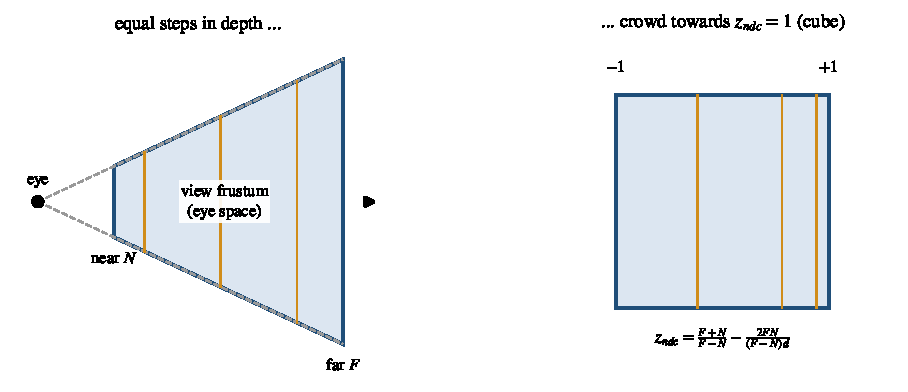
\includegraphics[width=\linewidth]{figures/diagrams/d_frustum_ndc.pdf}
\caption{The perspective divide squeezes the frustum into the NDC cube: slices equally spaced in depth (orange) crowd towards the far face, which is why depth precision is best near the camera (Eq.~\ref{eq:ndc}).}
\label{fig:d-ndc}
\end{figure}

\begin{figure}[htbp]
\centering\plot{p_depth_precision}{\linewidth}
\caption{Depth mapping of the scene's projection ($F=600$\,m, Eq.~\eqref{eq:ndc}): (a) window depth against
distance, (b) the smallest depth step.}
\label{fig:depth}
\end{figure}

With $N=0.05$\,m half of the depth range is used in the first 0.1\,m (Figure~\ref{fig:depth}a), and at 100\,m two
surfaces closer than about 1\,m cannot be ordered (b). Raising $N$ to 0.5\,m gains a factor of ten everywhere; this is
the z-fighting trade-off of Section~\ref{sec:hard}.
\begin{figure}[htbp]
\centering
\begin{subfigure}{0.49\linewidth}\raw{v5/scene_depth}{\linewidth}\caption{\key{F}: linearised Z-buffer view.}\end{subfigure}\hfill
\begin{subfigure}{0.49\linewidth}\raw{lab/explorer_stage_02_vertex}{\linewidth}\caption{Frame Explorer: vertex stage (clip space).}\end{subfigure}
\\[1mm]
{\footnotesize\textit{Zoomed panels of the Frame Explorer frame:}}\\[0.5mm]
\feStageVertexInfo\hfill\feStageVertexFormula
\caption{Depth in the renderer: (a) linearised depth ($d$ recovered from $z_w$ by inverting Eq.~\eqref{eq:ndc}; raw
$z_w$ would be almost white beyond a few metres), (b) the vertex stage in clip space.}
\label{fig:zbuf}
\end{figure}

\textbf{Limitation.} The near plane of 0.05\,m exists so a first-person rifle and a soldier's own hands are not clipped. It costs
depth precision far away (Figure~\ref{fig:depth}b). Reversed-Z with a floating-point depth buffer would remove the
problem but needs \code{glClipControl} (OpenGL 4.5), which the 3.3 baseline does not have.
